\documentclass[journal ]{new-aiaa}
\usepackage[utf8]{inputenc}
\usepackage{textcomp}
\usepackage{subcaption}
\usepackage{float}

\usepackage{graphicx}
\usepackage{amsmath}
\usepackage[version=4]{mhchem}
\usepackage{siunitx}
\usepackage{longtable,tabularx}
\setlength\LTleft{0pt} 

\title{Optimization of Multiple Rotors}

\author{J. Spencer \footnote{Undergraduate Researcher, Brigham Young University FLOW Lab.}}
\affil{Brigham Young University, Provo, Utah, 84601} 

\begin{document}

\maketitle

\begin{abstract}

This report describes a project completed as part of my research for the Brigham Young University FLOW Lab to discover ideal conditions for airfoil performance. Computational stimulations of propellors allow researchers to perform low-risk studies and develop designs more quickly. This investigation found the optimal chord length magnification and the optimal rotation angle for a rotor's efficiency. This was done with a computational simulation in the Julia programming language. This paper defines the operating conditions used in this optimization, presents rotors that were optimized at several blade counts, and discusses areas of possible future development in this research. This paper found that for the operating conditions used, rotors with the cord reduced to the optimization's lower limit, 50 percent, with slight negative twist angles were the most efficient. These results could be applied to rotors designed to produce the maximum output power for a given input power requirement, without regard to other conditions like the thrust or torque coefficients. Future work could combine these findings with other conditions to find the most efficient rotor that can also provide a required amount of thrust or operate at a variety of different rotational velocities.

\end{abstract}


\section*{Nomenclature}

{\renewcommand\arraystretch{1.0}
\noindent\begin{longtable*}{@{}l @{\quad \quad} l@{}}

$J$ & Advance Ratio \\
$\alpha$ & Angle of Attack (radians) \\
$\phi$ & Angle of Rotation (radians) \\
$M_{b}$ & Bending Moment (N$\cdot$m) \\
$c$ & Chord length (m) \\
$D$ & Diameter (m) \\
$c_{d}$ & Drag Coefficient \\
$\eta$ & Efficiency \\
$\rho$ & Fluid Density (kg/m$^{3}$) \\
$v_{\infty}$ & Freestream Velocity (m/s) \\
$c_{l}$ & Lift Coefficient \\
$C_{P}$ & Power Coefficient \\
$RPM$ & Revolutions Per Minute \\
$\sigma$ & Rotor Solidity \\
$C_{T}$ & Thrust Coefficient \\
$C_{Q}$ & Torque Coefficient \\

\end{longtable*}}


\section{Introduction}

\lettrine{P}{ropellors} come in a variety of different shapes and sizes. This paper describes how one propellor, a NACA 4412 airfoil attached to an APC 10x7 rotor, was optimized to perform more efficiently at a specific advance ratio. Because different blade counts could be more appropriate for different applications, blade counts of one, two, and three were each optimized and are compared in this report. This report produced useful code that could be applied to different rotors in the future.

\subsection{Context}

Computer simulations are very useful for modeling propellors. It would require significant investment of time, space, and money to perform an optimization like this, in which hundreds of slightly different propellors are compared. The first potential-flow codes, programs for modeling the pressure distribution of rotors, were developed in the 1960s and 1970s. Xfoil, the program used in this project, was first developed by MIT in the 1980s, with its current version dating to 2013. Xfoil.jl is the Julia wrapper used in this project, developed by Taylor McDonnell.\footnote{More information about both Xfoil and Xfoil.jl is available at \url{https://flow.byu.edu/Xfoil.jl/stable/} and \url{https://en.wikipedia.org/wiki/XFOIL}}

\subsection{Paper Outline} 

This paper first reviews the procedure used in the rotor optimization, including the equation used in the optimization and the initial conditions and constraints applied. Next, it reviews the results and compares them with each other. Finally, it draws conclusions based on the results of this experiment and discusses their meaning. All code used for each section of this report can also be accessed through a GitHub repository.\footnote{This repository can be accessed in the Rotor-Design branch of \url{https://github.com/JoeSpencer1/497R-Projects/tree/Final-Report}}


\section{Procedure}

This project was performed using Julia programming language.\footnote{Julia is available at \url{https://julialang.org}.} Jula is available for free and is useful for a variety of reasons. Like other languages, it can easily store data in vectors and perform rapid calculations with these objects. It is compiled just-in-time at runtime, which makes it run faster than interpreted languages like python without needing to be totally compiled before running like C. Being compiled just-in-time makes Julia faster than interpreted languages like python. Julia  packages, including those used during this semester, are also easily available from a package manager.\footnote{This article describes some of the benefits of Julia. \url{https://towardsdatascience.com/5-ways-julia-is-better-than-python-334cc66d64ae}}

\subsection{Computer Code}

Some Julia packages used for this project include Xfoil.jl,\footnote{Xfoil.jl is available at \url{https://github.com/byuflowlab/Xfoil.jl}} CCBlade,jl,\footnote{CCBlade.jl is available at \url{https://github.com/byuflowlab/CCBlade.jl}} and SNOW.jl.\footnote{SNOW.jl is available at \url{https://github.com/byuflowlab/SNOWl.jl}} Xfoil.jl analyzes the lift, drag, and moment coefficients of an airfoil from its geometry and angle of attack, and CCBlade.jl calculates a rotor's thrust, power, and efficiency\cite{CCBlade}. This investigation used SNOW.jl to repeat itself until it converged on an optimal solution.

\subsection{Design Constraints}

In the rotor design, the rotor is created and evaluated using Xfoil.jl and CCBlade.jl, as described previously. Data about the rotor, including its loads in the normal and tangential directions and its torque, were recorded. This data was then multiplied by a safety factor of $n=1.1$ to determine the maximum allowable loads before the rotor would break or a different material would be required. $n=1.1$ was the safety factor defined in the project prompt, but it was included in the code as an optional argument that could be adjusted for other circumstances. After constraints were determined, rotor variable types called \emph{rotortest} were created with variable chord thickness magnification and rotation angle and the program used SNOW.jl to find the rotor with the optimal twist angle and chord thickness magnification for the objective function.

The objective function used in this optimization is very simple, as shown in equation~\eqref{equation:1}. 

\begin{equation}
	\begin{aligned}
	\label{equation:1}
	f(x_{1}, x_{2}, x_{3}...) = \eta \\
	\end{aligned}
\end{equation}.

In addition to restrictions on the moment and torque mentioned previously, the cord thickness was kept within a factor of two of the original and the twist angle was kept between $-90^{\circ}$ and $90^{\circ}$. These constraints are listed in table~\eqref{tab:2}. They ensured that the optimization found a reasonable solution confined to real limits, shown in table~\eqref{tab:2}.

\begin{center}
\label{tab:2}
\begin{tabular}{l  r}
	 \multicolumn{2}{c}{Table I: Optimization objective, parameters, and constraints}  \\ \hline
  	Maximize: & $\eta$ \\ \hline
  	By varying: & scale of the chord, $c$ \\ 
  	 & twist angle, $\phi$ \\  \hline
  	Subject to & total torque $\leq$ 110\% original \\ 
	 & normal moment $\leq$ 110\% original \\ 
	 & tangential moment $\leq$ 110\% original \\ 
	 & $-90^{\circ} <$ twist angle $< 90^{\circ}$ \\
	 & $50\% <$ chord magnification $< 200\% $ \\ \hline
\end{tabular}
\end{center}

The optimized rotors each had other features in common between them, shown in the last entry of table~\eqref{tab:4}. Ning (page 200) stated that the advance ratio is available from other variables already listed in the table by equation~\eqref{equation:3}, in which $v_{\infty}$ is the free stream velocity, $n$ is the rotational velocity in revolutions per second, and $D$ is the outer diameter \cite{ComAer}.

\begin{equation}
	\begin{aligned}
	\label{equation:3}
	J = \frac{v_{\infty}}{n D}
	\end{aligned}
\end{equation}

\begin{center}
\begin{tabular}{| c | c | c | c |}
	\multicolumn{4}{c}{Table II: Input value limits in rotor design} \\ \hline
  	 \textbf{Parameter} & \textbf{Default Value} & \textbf{Minimum Value} & \textbf{Maximum Value} \\ \hline
	 Chord Length, & 100\% length & 50\% & 200\% \\ \hline
	 Twist Angle, & $0^{\circ}$ & $-90^{\circ}$ & $90^{\circ}$ \\ \hline \hline
	 Rotational Velocity, $RPM$ & \multicolumn{3}{c|}{6000 RPM} \\ \hline
	 Blade Count & 2 blades & \multicolumn{2}{c|}{1 to 3)}\\ \hline
	 Hub-to-tip ratio & \multicolumn{3}{c|}{10\%} \\ \hline
	 Air Density & \multicolumn{3}{c|}{1.225 kg/$m^{3}$} \\ \hline
	 Diameter & \multicolumn{3}{c|}{0.254 m (10 in.)} \\ \hline
	 Velocity & \multicolumn{3}{c|}{12 m/s (26.84 mph)} \\ \hline
	 Advance Ratio & \multicolumn{3}{c|}{0.472} \\ \hline
\end{tabular}
\label{tab:4}
\end{center}

\section{Optimization}

The objective function, equation~\eqref{equation:1}, was optimized using SNOW.jl. The code was designed so that SNOW.jl found the maximum by finding the minimum of its negative. This is similar to the technique and sign convention described by Martins and Ning in page 10 of Engineering Design Optimization \cite{EngDesOpt}.


\section{Results}

Although the chord thickness changed during the optimization for all blade counts, both the rotor identification and the NACA number stayed the same throughout the optimization. Changing the pitching angle only rotated the rotor blade, and changing the chord length magnified the size of its entire profile uniformly.

\subsection{Results Plot}

Figure~\eqref{fig:5} shows that while the optimized design increased the efficiency of even the rotor with a higher blade count above the rotor pre-optimization, it dramatically decreases the thrust and torque coefficients. The efficiency at higher advance ratios also decreased. These decreases in other rotor properties may not be desired. This illustrates one problem with optimizers: if created correctly, they will do exactly what they are programmed to do and may sacrifice some desirable properties to further optimize the objective function.

\begin{figure}[H]
\centering
 	\subfloat[Efficiency]{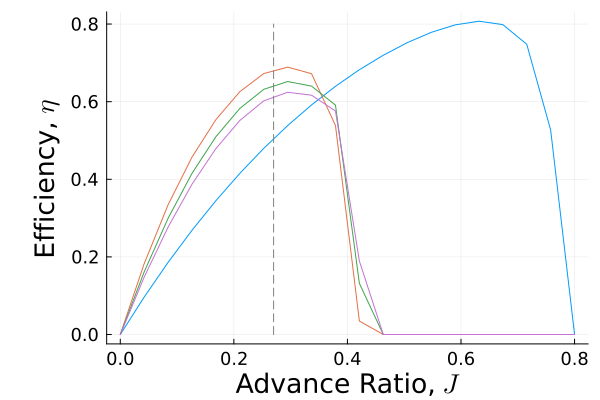
\includegraphics[width = .35\textwidth]{Plots/Figure_1.png}}
	\subfloat[Thrust Coefficient]{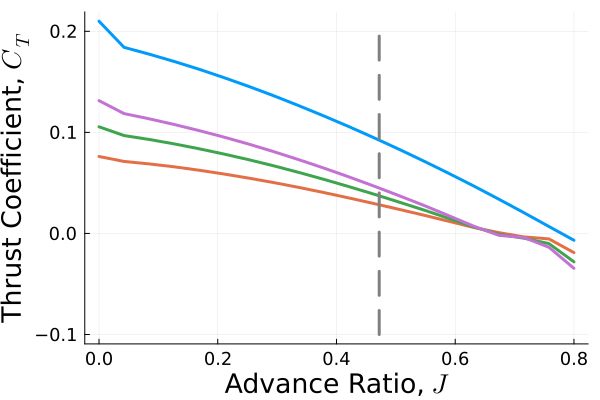
\includegraphics[width = .35\textwidth]{Plots/Figure_2.png}}

	\subfloat[Torque Coefficient]{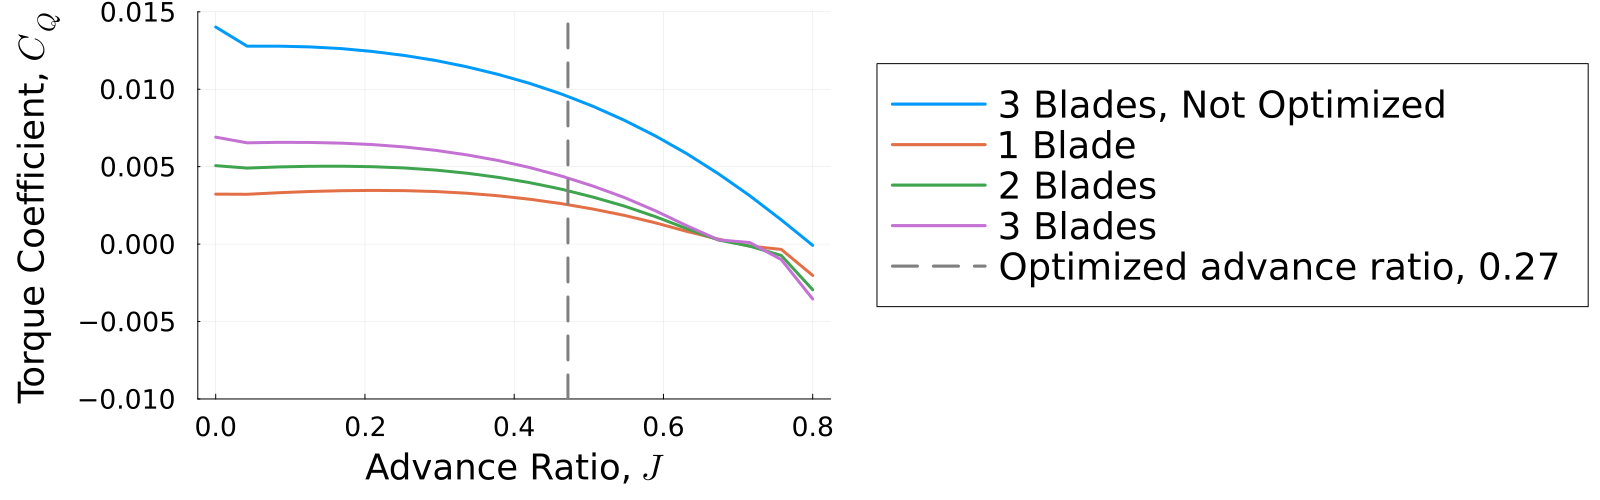
\includegraphics[width = .70\textwidth]{Plots/Figure_3.png}}\hspace{1em}
	\caption{Efficiency, Thrust Coefficients, and Torque Coefficients Compared at Different Advance Ratios}
	\captionsetup{aboveskip=0pt,font=it}
	\label{fig:5}
\end{figure}

If necessary, minimum thrust and torque coefficients could be provided as parameters along with the maximums shown below the objective function in table~\eqref{tab:2}. These could find the angle of rotation and chord thickness that would provide the maximum efficiency while still maintaining some required thrust. The optimizer might not reduce the rotor to its minimum possible chord thickness in every case as it did in this optimization.

\subsection{Results Table}

Table~\eqref{tab:6} shows the optimal twist angles and chord magnifications for each different rotor blade count. At the conditions listed in table~\eqref{tab:4}, the optimal chord length magnification was constant, and the optimal angle of rotation was less than $-3^{\circ}$ for each rotor. It gradually became more negative as the blade count increased.

\begin{center}
\begin{tabular}{| c | c | c |}
	 \multicolumn{3}{c}{Table III (Table IV.B): Optimized chord magnification and rotation angles for different blade counts}  \\ \hline
  	 \textbf{Blade Count} & \textbf{Chord Thickness Multiplication} & \textbf{Twist Angle} \\ \hline
  	 3 (Default) & 1.0 & $0^{\circ}$ \\ \hline
  	 2 & 0.50 & $-2.70^{\circ}$ \\ \hline
  	 3 & 0.50 & $-2.88^{\circ}$ \\ \hline
  	 4 & 0.50 & $-2.94^{\circ}$ \\ \hline
\end{tabular}
\label{tab:6}
\end{center}


\section{Discussion}

The propellor was checked at blade counts of 1, 2, and 3. These results found that for all three blade counts, the optimal propellor was as thin as possible, with a small negative angles of attack. The finding about thinner rotor blades being more efficient agreed with Saraf, Nouli, Ravalet, and Bakir's findings, but the negative rotation angle was surprising at first \cite{AxFlFan}.

One lesson learned from this optimization is that the user should be careful what is optimize for, because the computer will optimize exactly what it is told, even if that is not what the user actually wants. An optimization that is written incorrectly or has unseen loopholes can not only give a misleading answer but also waste a lot of time. In the case of this optimization, I think other constraints could have been added to the optimization

\subsection{Efficiency Equation}

One problem with this optimization is that a rotor's efficiency is available as a function of the advance ratio, the thrust coefficient, and the power coefficient. The equation for efficiency is described by Andrew Ning in \emph{Computational Aerodynamics}, page 200 \cite{ComAer} using the relation below, equation~\eqref{equation:7}.

\begin{equation}
	\begin{aligned}
	\label{equation:7}
	\eta = J \frac{C_{T}}{C_{P}}
	\end{aligned}
\end{equation}

With $J$ kept constant, as it was in this research, this equation can be maximized in either by maximizing $C_{T}$ or by minimizing $C_{P}$, which is equal to $C_{Q}$ multiplied by $2 \pi$. Inspection of figure~\eqref{fig:5} reveals that the optimizer did the latter. The torque coefficient $C_{Q}$ is significantly lower for each rotor. While the thrust coefficient $C_{T}$ did not decrease by as much as $C_{Q}$, it is still much lower than before. Although more efficient, the newly optimized propellor has a much lower solidity and is better suited for a different environment.

\subsection{Angle of Rotation}

The optimal angles of rotation were between $-2.70^{\circ}$ and $-2.94^{\circ}$, as shown in table~\eqref{tab:6}. These negative angles of rotation were surprising at first, because angles near $0^{\circ}$ were expected to be the most efficient. Figure~\eqref{fig:8}, from airfoil analysis conducted earlier in the semester, shows that $0^{\circ}$ angles of attack do not necessarily correspond to the lowest lift and drag coefficients for the NACA 4412 airfoil used in this design. Although that finding was for more simple analysis of an airfoil, it was concluded that a negative angle of rotation was possible.

\begin{figure}[H]
\centering
 	\subfloat[Lift Coefficient]{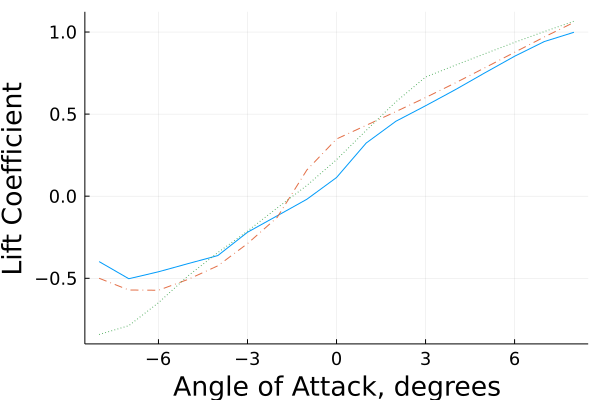
\includegraphics[width = .35\textwidth]{Plots/Figure13.png}}
	\subfloat[Drag Coefficient]{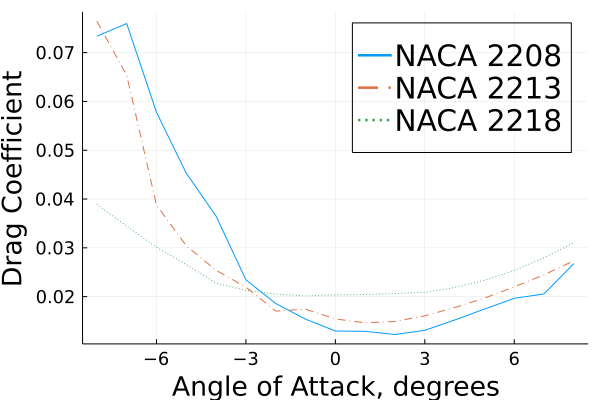
\includegraphics[width = .35\textwidth]{Plots/Figure14.png}}
	\caption{Lift and Drag Experienced by NACA 4412 Airfoils}
	\captionsetup{aboveskip=0pt,font=it}
	\caption*{These plots show how lift and drag change for an airfoil at different angles of attack.}
	\label{fig:8}
\end{figure}


\section{Conclusion}

This optimization combined several different Julia packages to find the optimal angle of rotation and rotor chord length for a rotor's efficiency. It found that rotors with very small chord lengths at negative angles of rotation were the most efficient. Other optimizations could be performed by simple editing of the code used in this research to find which rotors perform best in other applications or environments. 


\section{Acknowledgements}

The author would like to thank Adam Cardoza for mentoring him in learning the codes used in the FLOW Lab, directing his research, helping him through questions and challenges that he discovered during his work.



\bibliography{Final_Report}

\end{document}
